B-Tree and its variants have been widely used as indexes in
databases. For example, the PostgreSQL uses B-Tree as its index. B-Trees
can be considered as a natural generalisation of binary search tree. In
binary search tree, there is only one key and two possible children in
the internal node. However, an internal node of B-Tree can contain
several keys and children. The keys in a node serve as dividing points
and separate the range of keys. With this structure, we make a
multi-way decision based on comparisons with the keys stored at the node
$x$. The image below illustrates a simple B-Tree.

In this section, we introduce the construction and query processes
of B-Trees and then analyse their properties.

\subsubsection{Motivation}

In computers, the memories are organised in an hierarchical way. For example, a classical computer system consists three layers of memory: the CPU cache, main memory and the hard disk. In such a system, the CPU cache is the fastest but the most expensive while and hard disk is the cheapest but also the slowest. When querying for an item, the CPU will first try to fetch it from the CPU cache. If not there the CPU will then try to fetch it from the main memory, and then the hard disk.

%TODO: Some statements are needed to show the data is stored in blocks in the memory.

At the same time, the traditional hard disk drive (HDD) is made by a moving mechanical structure.

%TODO: Illustrate the mechanical structure.
% Should we be writing this since we are using in-memory ?

In summary, there are two properties in classical computer systems that we need to take into account:

\begin{enumerate}
	\item The memory is not flat, meaning that memory references are not equally expensive. 
	\item 
\end{enumerate}

\subsubsection{Definition and Terms}
\begin{figure}[htp]
    \centering
    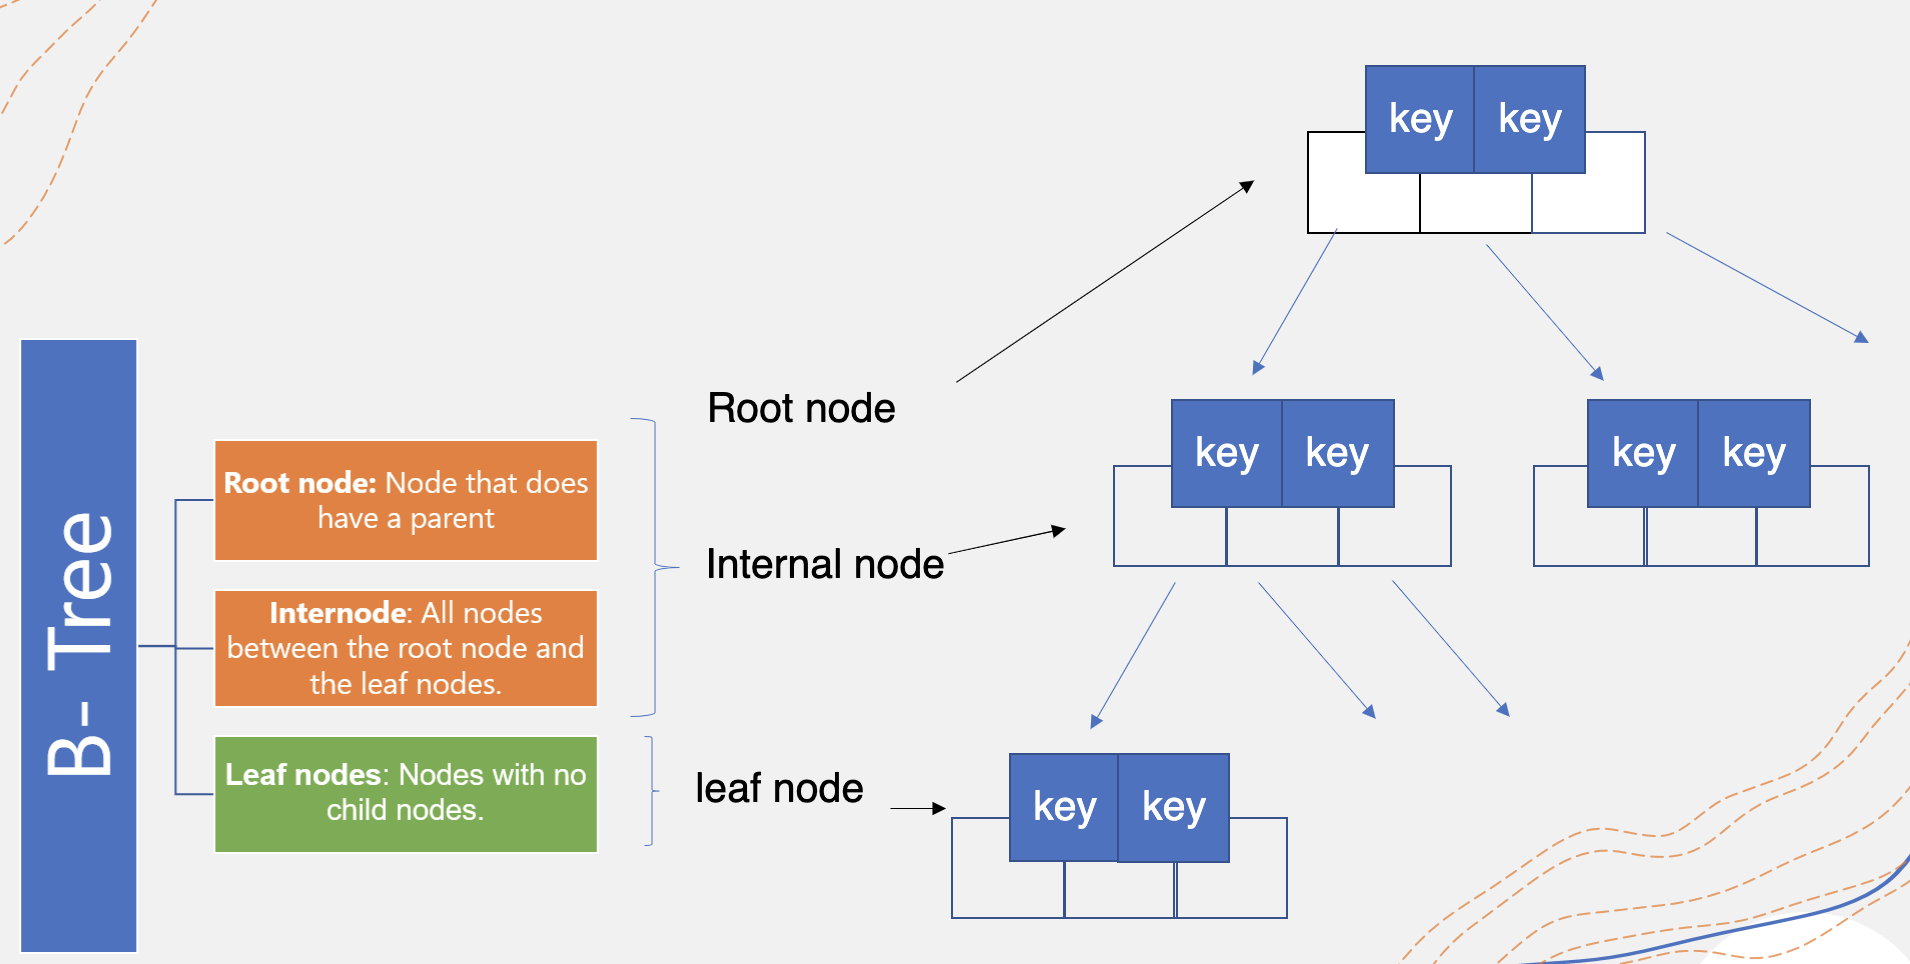
\includegraphics[width=0.6\textwidth]{graphs/B-Tree_definitions.png}
    \caption{B-Tree}
    \label{fig:B-Tree}
\end{figure}

Before we formally define B-Trees, we assume the following terms:

\begin{itemize}
\item
  \textbf{Keys}: The key in a database is a special attribute that could identify a row in the database. In our work, each key corresponds to a 1-dimensional
  \textbf{value} and forms a key-value pair.
\item
  \textbf{Order}: The Order of a B-Tree is the maximum number of children that a node can have. Number of keys in a node is always one less than the order of the tree at the maximum.
\item
  \textbf{Internal Node}: An internal node is any node of the tree that has child nodes and is not a root node.
\item
  \textbf{Leaf Node}: A leaf node is any node that does not have child nodes.
\end{itemize}

Each node in a B-Tree has the following attributes:

\begin{itemize}
\item
  $x.n$ is the number of keys currently stored in the node $x$.
\item
  Inside each node, the keys are sorted in non decreasing order, so that
  we have $x.keys_1\leq x.keys_2\leq\cdots\leq x.keys_{x.n}$.
\item
  $x.leaf$, a Boolean value determines if current node is a leaf node.
\end{itemize}

With these properties, A B-Tree $T$ whose root is $T.root$ have the
following properties:

\begin{itemize}
\item
  Each internal node $x$ contains $x.n+1$ children. We assume the
  children are $x.c_1,\cdots,x.c_{x.n+1}$.
\item
  The nodes in the tree have lower and upper bounds on the number of
  keys that can contain. These bounds can be expressed in terms of a
  fixed integer $t$.
\end{itemize}

\subsubsection{Insertion of B-Tree}

When inserting keys into a binary search tree, we search for the leaf
position at which to insert the new key. However, with B-Tree, we cannot
simply find the position, create a new node and insert the value because
the tree will be imbalanced again. Hence, in this section, we illustrate
an operation that splits a full node around its median key

\begin{algorithm}[H]
    \SetAlgoLined
    \SetKwInOut{Input}{Input}
     \Input{\texttt{$m$:order\_of\_tree ,$(k,v)$:(key, value), $N$:Node;}}
    \SetKwInOut{Output}{Output}
     \Output{\texttt{B-Tree}}
     \eIf{$N$ is a leaf and not yet full}  
     {
        \texttt{insert $(k,v)$ into $N$}
     }
     {
        \texttt{create new Node N'}\\
        \texttt{Find the median of the node}\\
        \texttt{Add the value at the median location to the new node N'}\\
     }
    \If{$N$ is root with no children and not full}
    {
    
        \texttt{insert $(k,v)$ into $N$}
        
    }
     \caption{Algorithm for B-Tree insertion}
     \label{B-Tree Insertion}
\end{algorithm}


\begin{figure}[htp]
    \centering
    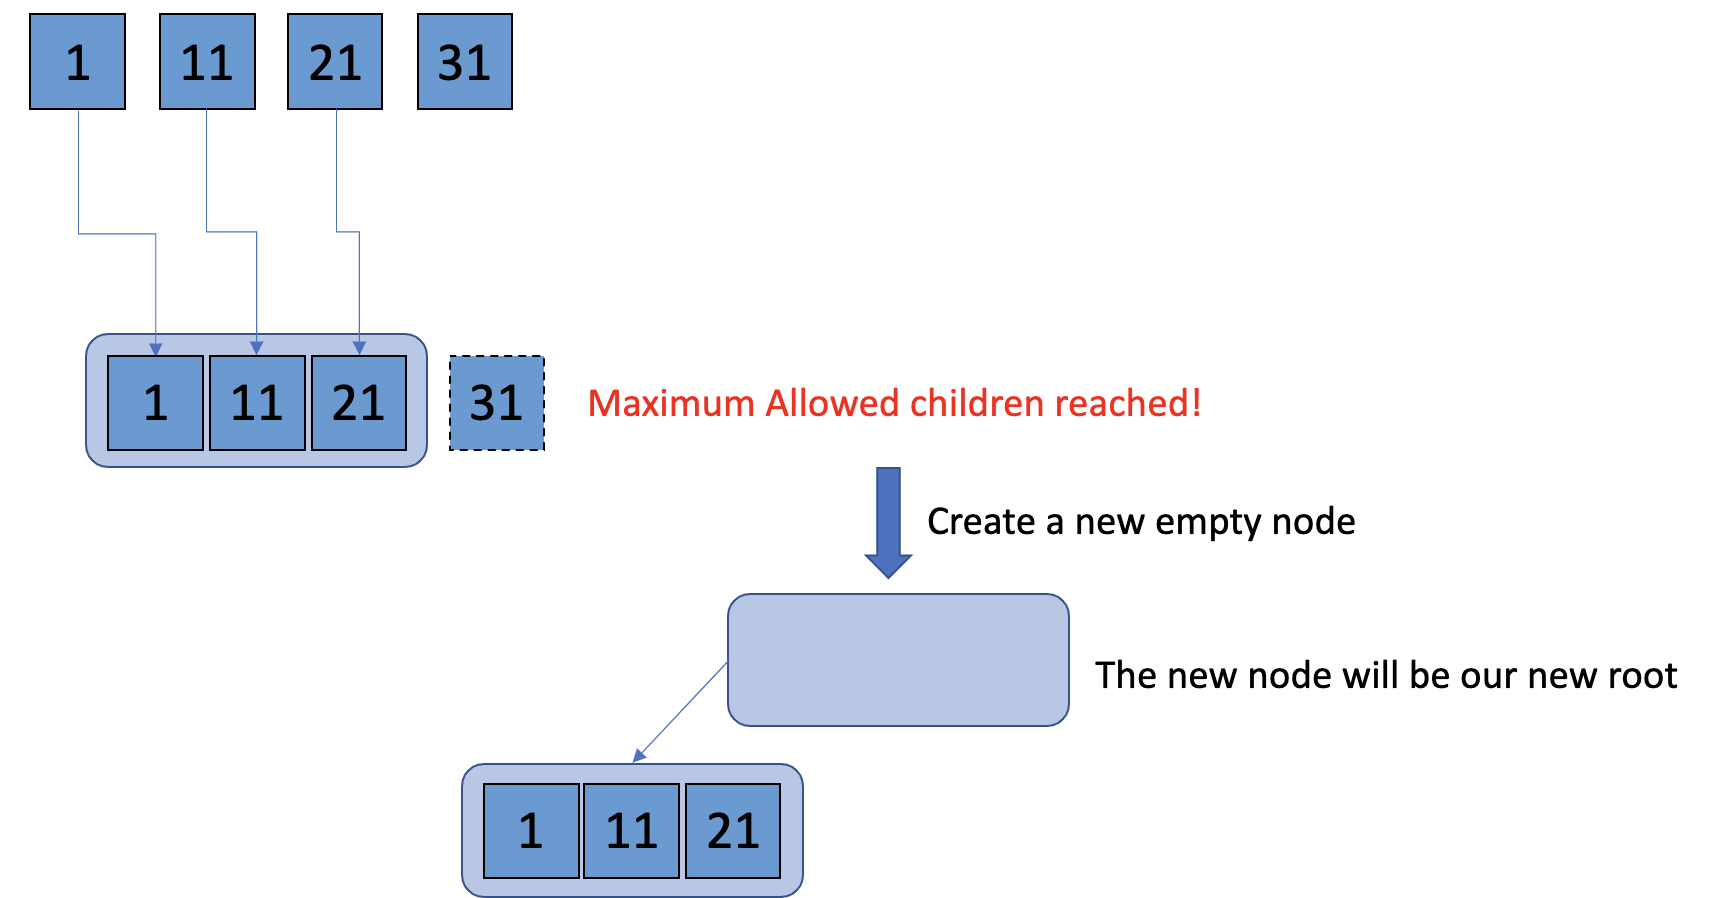
\includegraphics[width=0.6\textwidth]{graphs/B-Tree_example01.png}
    \caption{B-Tree key insertion}
    \label{fig:B-Tree key insertion1}
\end{figure}

\begin{figure}[htp]
    \centering
    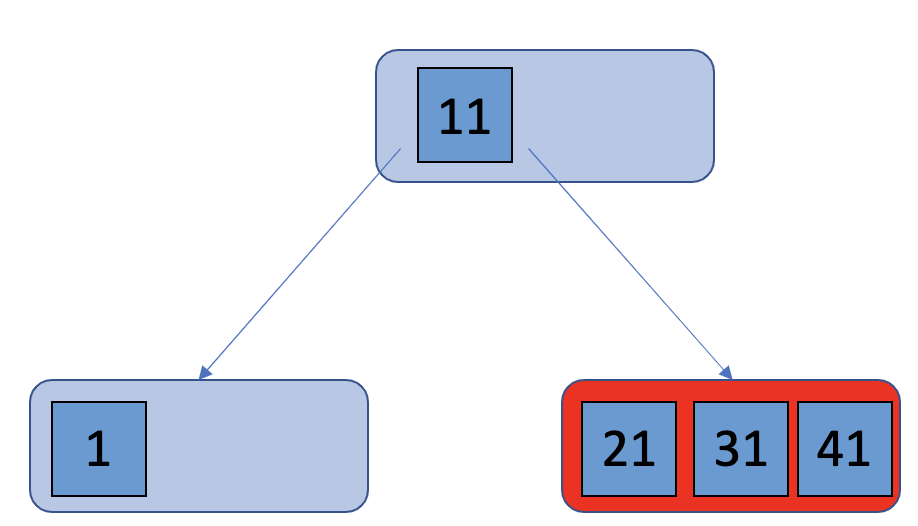
\includegraphics[width=0.3\textwidth]{graphs/B-Tree_example02.png}
    \caption{B-Tree key insertion}
    \label{fig:B-Tree key insertion2}
\end{figure}

\subsubsection{Insertion in a B-Tree}

There are two conditions in insertion:
\begin{itemize}
\item
\textbf{When the node is empty or not created at all}:
In the algorithm, initially when the first key is inserted and there is no root to the tree it will check the condition if there are any nodes and if not create a new one. It will insert the new key in the node and keeps inserting the new keys until it is one less than the order of the B-Tree being created. 
\item
\textbf{When the node is full}:
As soon as the maximum number of allowed children has reached for the root node a new empty node is created. Suppose we have inserted [1,11,21] to a node of a B-Tree with degree 4. Now if we want to insert a new value 31 into the tree, since it has reached the maximum number of children it will find the median of the existing node [1,11,21] which is 11 and increase the level of the B-tree to 2 and make [1] and [21] child nodes of [11]. So now if a new value is to be inserted it can be inserted. Splitting of the node happens each time it reaches it's maximum allowed keys. Now 31 will be compared with 11 and since 31 > 11 it will be inserted in the right child and it will have an updated value of [21,31]. More keys can then be inserted until it reaches it's maximum and splits again. Once the node is split it's parent is also updated to the median value i.e., [11] in this case for nodes [1] and [21,31,41] as can be seen in \ref{fig:B-Tree key insertion2}.
\end{itemize}

\subsubsection{Search in a B-Tree}

\begin{algorithm}[H]
    \SetAlgoLined
    \SetKwInOut{Input}{Input}
     \Input{\texttt{k ; key, root ; Root of the B-Tree}}
    \SetKwInOut{Output}{Output}
     \Output{\texttt{Value associated with key}}
     \For{$i\gets0$ \KwTo $len(Root Node)$}{
         \If{keys in root greater than k}
         {
            \texttt{SEARCH\_CHILD(key)} //Search linearly the child associated with the key location one before\\
            \eIf{Child is a leaf}
            {
                \texttt{Linearly search until the key is reached}
            }
            {
                \texttt{SEARCH\_CHILD(key)}
            }
            
         }
    }
     \caption{Algorithm for B-Tree Search}
     \label{B-Tree Search}
\end{algorithm}

Search in a B-Tree is basically the comparison of the value of the key that needs to be searched with the keys in the node. It first linearly checks the value in the root key and looks for a key value which is greater than the searched key. As soon as it finds a key greater than the searched key it will search in the child of the key before it. For example if we were to search of key [41] in the example of the B-Tree used above, we would first check the value [11] and since it smaller than [31] and there are no keys greater than this in the root node it will search in the right child of the root node. It will then linearly search the node and locate it's associated value and return it. 